\documentclass{article}
\usepackage{graphicx} 
% Graphics and diagrams
\usepackage{tikz}

% Required TikZ libraries
\usetikzlibrary{
    arrows.meta,
    positioning,
    fit,
    shapes.geometric
}% Required for inserting images

\title{Spectrum analyser}
\author{Ansh Gupta & Shubham }
\date{September 2026}
\documentclass[12pt,a4paper]{article}

% -------------------------------------------------
% PACKAGES
% -------------------------------------------------
\usepackage[margin=1in]{geometry}
\usepackage{graphicx}
\usepackage{booktabs}
\usepackage{array}
\usepackage{float}
\usepackage{amsmath}
\usepackage{amssymb}
\usepackage{caption}
\usepackage{listings}
\usepackage{xcolor}
\usepackage[
    bookmarks,
    breaklinks,
    colorlinks=true,
    linkcolor=black,
    citecolor=black,
    urlcolor=black
]{hyperref}
\usepackage{enumitem}

% -------------------------------------------------
% PAGE SETTINGS
% -------------------------------------------------
\setlength{\parindent}{0pt}
\setlength{\parskip}{0.8em}

% -------------------------------------------------
% CODE STYLE
% -------------------------------------------------
\definecolor{codegray}{RGB}{245,245,245}

\lstset{
    backgroundcolor=\color{codegray},
    basicstyle=\ttfamily\small,
    breaklines=true,
    frame=single,
    numbers=left,
    numberstyle=\tiny,
    numbersep=8pt,
    keywordstyle=\color{blue},
    commentstyle=\color{green!50!black},
    stringstyle=\color{red!60!black}
}

% -------------------------------------------------
% DOCUMENT
% -------------------------------------------------
\usepackage{graphicx} 
% Graphics and diagrams
\usepackage{tikz}

% Required TikZ libraries
\usetikzlibrary{
    arrows.meta,
    positioning,
    fit,
    shapes.geometric
}% Required for inserting images

\title{Spectrum analyser}
\author{Ansh Gupta & Shubham }
\date{September 2026}
\documentclass[12pt,a4paper]{article}

% -------------------------------------------------
% PACKAGES
% -------------------------------------------------
\usepackage[margin=1in]{geometry}
\usepackage{graphicx}
\usepackage{booktabs}
\usepackage{array}
\usepackage{float}
\usepackage{amsmath}
\usepackage{amssymb}
\usepackage{caption}
\usepackage{listings}
\usepackage{xcolor}
\usepackage[
    bookmarks,
    breaklinks,
    colorlinks=true,
    linkcolor=black,
    citecolor=black,
    urlcolor=black
]{hyperref}
\usepackage{enumitem}

% -------------------------------------------------
% PAGE SETTINGS
% -------------------------------------------------
\setlength{\parindent}{0pt}
\setlength{\parskip}{0.8em}

% -------------------------------------------------
% CODE STYLE
% -------------------------------------------------
\definecolor{codegray}{RGB}{245,245,245}

\lstset{
    backgroundcolor=\color{codegray},
    basicstyle=\ttfamily\small,
    breaklines=true,
    frame=single,
    numbers=left,
    numberstyle=\tiny,
    numbersep=8pt,
    keywordstyle=\color{blue},
    commentstyle=\color{green!50!black},
    stringstyle=\color{red!60!black}
}

% -------------------------------------------------
% DOCUMENT
% -------------------------------------------------
\begin{document}

% -------------------------------------------------
% TITLE PAGE
% -------------------------------------------------

\begin{center}

\vspace*{1cm}

\begin{figure}
  \centering
  \begin{minipage}{7cm}
    
\includegraphics[scale=1.2]{cedtnew.png}
  \end{minipage}
\end{figure}

\vspace{-2cm}

\subsection*{
\hspace{2.2cm}Centre\hspace{0.25cm}for\hspace{0.25cm}
Electronic\hspace{0.25cm}Design\hspace{0.25cm}
and\hspace{0.25cm}Technology
}

\subsection*{
\hspace{1.3cm}Netaji\hspace{0.25cm}Subhas\hspace{0.25cm}
University\hspace{0.25cm}of\hspace{0.25cm}
Technology\hspace{0.25cm},\hspace{0.25cm}
New\hspace{0.15cm}Delhi
}

\vspace{10cm}



\begin{center}


\textbf{\huge Real-Time Audio Spectrum Analyzer}\\[1cm]

{\large \textbf{Submitted by}}\\[0.2cm]

{\large Shubham }\\

\vspace{0.8cm}

{\large \textbf{Date:} February 2025}

\end{center}

\end{spacing}



\thispagestyle{empty}

% -------------------------------------------------
% TABLE OF CONTENTS
% -------------------------------------------------
\newpage
\tableofcontents
\newpage

% -------------------------------------------------
% TABLE OF CONTENTS
% -------------------------------------------------



% =================================================
% 1 SYNOPSIS
% =================================================

\section{Synopsis}

This project implements a real-time audio spectrum analyzer using an Arduino microcontroller, an analog microphone sensor, and an OLED display. The system acquires an analog audio signal through the Arduino's Analog-to-Digital Converter (ADC), samples the signal at a rate of 10 kHz, and processes blocks of 128 samples using a Fast Fourier Transform (FFT).

Before performing the FFT, a Hann window is applied to the sampled data to reduce spectral leakage. The FFT converts the audio signal from the time domain into the frequency domain. The magnitude of each frequency bin is calculated, and the bin containing the maximum magnitude is identified as the dominant frequency component.

The detected FFT bin is converted into frequency in hertz and represented as an integer. The display subsystem receives this dominant frequency value and raises the corresponding frequency bar on the OLED display.

The project demonstrates the implementation of an embedded Digital Signal Processing (DSP) system involving real-time data acquisition, timer-based sampling, ADC operation, windowing, FFT computation, frequency extraction, and graphical visualization.

\newpage

% =================================================
% 2 INTRODUCTION
% =================================================

\section{Introduction}

Sound is a time-varying analog signal containing one or more frequency components. Although the waveform can be observed directly in the time domain, the individual frequencies present in the signal cannot be easily identified from the waveform alone.

A spectrum analyzer converts the signal from the time domain into the frequency domain and displays the distribution of signal energy across different frequencies.

The Fast Fourier Transform (FFT) is an efficient algorithm used to perform this conversion. Instead of analyzing the waveform only as:

\[
\text{Amplitude versus Time}
\]

the FFT represents it as:

\[
\text{Magnitude versus Frequency}
\]

This project uses an Arduino-based embedded system to implement real-time frequency analysis of an audio signal. An analog microphone sensor provides the input signal to the Arduino ADC. The samples are collected at a fixed sampling rate and stored in a buffer. Once a complete buffer is obtained, a Hann window is applied and a 128-point FFT is performed.

The frequency component with the highest magnitude is then identified. The corresponding FFT bin is converted into an integer frequency value and passed to an independent display function.

The project separates the system into two major functional blocks:

\begin{enumerate}
    \item \textbf{Digital Signal Processing Block}
    \begin{itemize}
        \item Sampling
        \item Windowing
        \item FFT
        \item Magnitude calculation
        \item Dominant frequency detection
    \end{itemize}

    \item \textbf{Display Block}
    \begin{itemize}
        \item Receive dominant frequency
        \item Determine corresponding display position
        \item Raise the corresponding frequency bar
    \end{itemize}
\end{enumerate}

This modular approach separates signal processing from visualization and improves the overall software structure.

\newpage

% =================================================
% 3 APPARATUS
% =================================================

\section{Apparatus}

\subsection{Hardware}

\begin{table}[H]
\centering
\caption{Hardware used in the project}
\begin{tabular}{|p{5cm}|p{8cm}|}
\hline
\textbf{Component} & \textbf{Specification / Purpose} \\
\hline

Microcontroller & Arduino Nano\\
\hline

Audio Sensor & KY-037 High Sensitivity Sound Microphone Sensor Module \\
\hline

Display & SSD1306 OLED Display \\
\hline


Connection Hardware & Breadboard and jumper wires \\
\hline

Power Supply & Arduino USB or regulated DC supply \\
\hline

\end{tabular}
\end{table}

\subsection{Software}

The following software and libraries are used:

\begin{itemize}
    \item Arduino IDE
    \item U8g2 graphics library
    \item \texttt{fix\_fft} library
    \item AVR program memory library
    \item AVR interrupt library
    \item SPI library
\end{itemize}

The program directly accesses the Arduino ADC and Timer1 registers instead of relying entirely on high-level functions such as \texttt{analogRead()}.

\newpage
% =================================================
% 4 BLOCK DIAGRAM
% =================================================

\section{Block Diagram}

The overall system architecture of the real-time audio spectrum analyzer is shown in Figure~\ref{fig:blockdiagram}.

\begin{figure}[H]
\centering

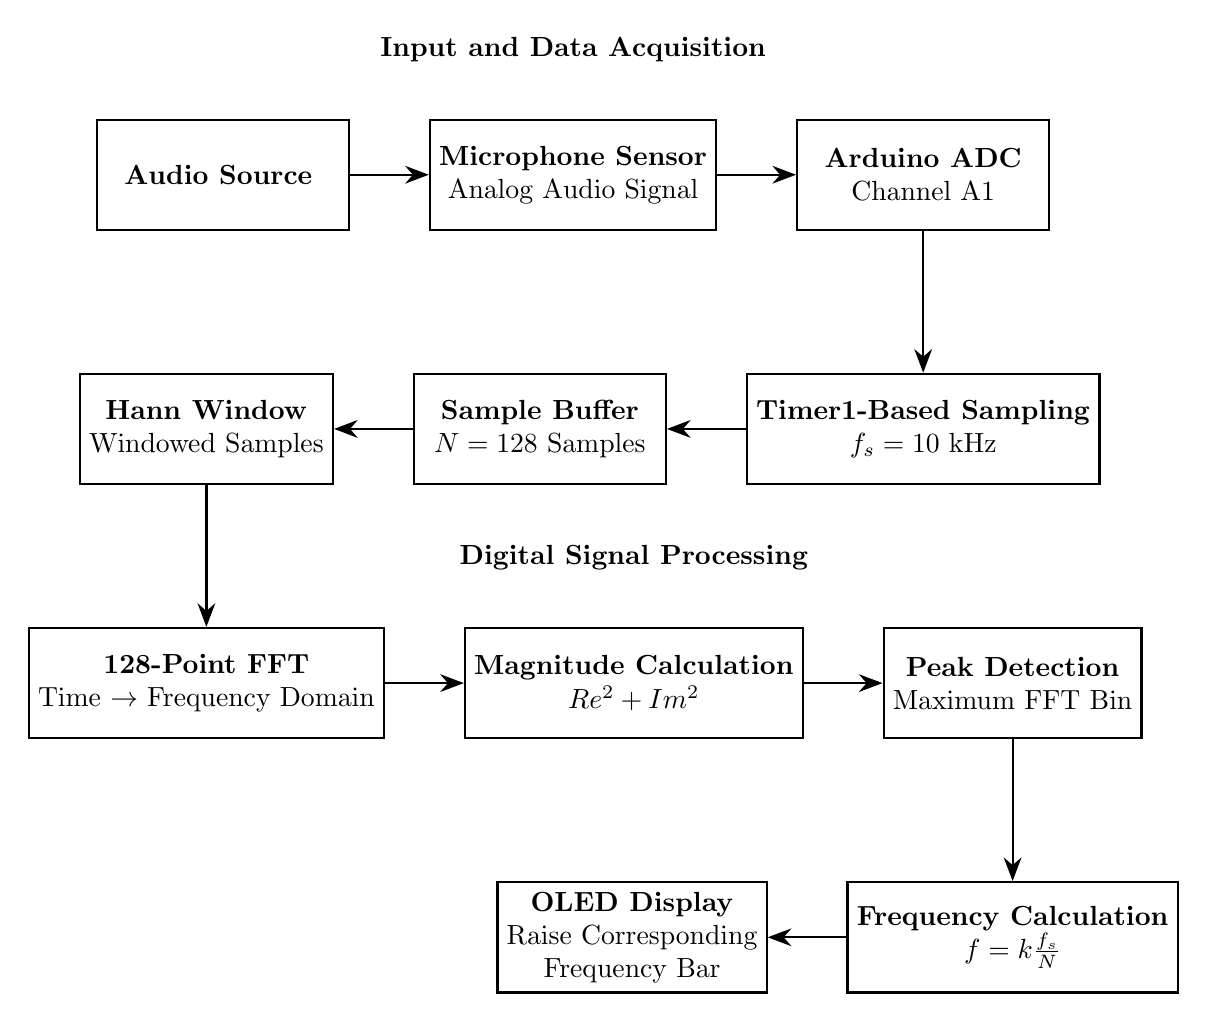
\begin{tikzpicture}[
    block/.style={
        rectangle,
        draw,
        thick,
        minimum width=3.2cm,
        minimum height=1.4cm,
        align=center
    },
    smallblock/.style={
        rectangle,
        draw,
        thick,
        minimum width=2.7cm,
        minimum height=1.2cm,
        align=center
    },
    arrow/.style={
        -{Stealth[length=3mm]},
        thick
    },
    node distance=1cm
]

% -------------------------------------------------
% FIRST ROW
% -------------------------------------------------

\node[block] (audio) {
    \textbf{Audio Source}
};

\node[block, right=of audio] (mic) {
    \textbf{Microphone Sensor}\\
    Analog Audio Signal
};

\node[block, right=of mic] (adc) {
    \textbf{Arduino ADC}\\
    Channel A1
};

% -------------------------------------------------
% SECOND ROW
% -------------------------------------------------

\node[block, below=1.8cm of adc] (sampling) {
    \textbf{Timer1-Based Sampling}\\
    $f_s = 10$ kHz
};

\node[block, left=of sampling] (buffer) {
    \textbf{Sample Buffer}\\
    $N = 128$ Samples
};

\node[block, left=of buffer] (window) {
    \textbf{Hann Window}\\
    Windowed Samples
};

% -------------------------------------------------
% THIRD ROW
% -------------------------------------------------

\node[block, below=1.8cm of window] (fft) {
    \textbf{128-Point FFT}\\
    Time $\rightarrow$ Frequency Domain
};

\node[block, right=of fft] (mag) {
    \textbf{Magnitude Calculation}\\
    $Re^2 + Im^2$
};

\node[block, right=of mag] (peak) {
    \textbf{Peak Detection}\\
    Maximum FFT Bin
};

% -------------------------------------------------
% FOURTH ROW
% -------------------------------------------------

\node[block, below=1.8cm of peak] (freq) {
    \textbf{Frequency Calculation}\\
    $f = k\frac{f_s}{N}$
};

\node[block, left=of freq] (display) {
    \textbf{OLED Display}\\
    Raise Corresponding\\
    Frequency Bar
};

% -------------------------------------------------
% SIGNAL FLOW ARROWS
% -------------------------------------------------

\draw[arrow] (audio) -- (mic);
\draw[arrow] (mic) -- (adc);

\draw[arrow] (adc.south) -- ++(0,-0.5) -| (sampling.north);

\draw[arrow] (sampling) -- (buffer);
\draw[arrow] (buffer) -- (window);

\draw[arrow] (window.south) -- ++(0,-0.5) -| (fft.north);

\draw[arrow] (fft) -- (mag);
\draw[arrow] (mag) -- (peak);

\draw[arrow] (peak.south) -- ++(0,-0.5) -| (freq.north);

\draw[arrow] (freq) -- (display);

% -------------------------------------------------
% STAGE LABELS
% -------------------------------------------------

\node[
    above=0.6cm of mic,
    font=\bfseries
] {Input and Data Acquisition};

\node[
    above=0.6cm of mag,
    font=\bfseries
] {Digital Signal Processing};

\end{tikzpicture}

\caption{Block diagram of the Arduino-based real-time audio spectrum analyzer}
\label{fig:blockdiagram}

\end{figure}

\newpage

% =================================================
% 5 PROCEDURE
% =================================================

\section{Procedure}

The following procedure was used to implement the spectrum analyzer.

\subsection{Audio Signal Acquisition}

An analog microphone sensor was connected to the Arduino analog input channel A1. The microphone converts sound pressure variations into an electrical analog signal.

\subsection{ADC Configuration}

The Arduino ADC was configured directly through the AVR registers.

The ADC reference voltage was set to AVcc, and ADC channel 1 was selected.

The ADC prescaler was configured to 64.

For a typical Arduino clock frequency of 16 MHz:

\[
f_{ADC} =
\frac{16\,\text{MHz}}{64}
\]

Therefore:

\[
f_{ADC} = 250\,\text{kHz}
\]

The ADC conversion was initiated directly through the ADC control register.

\subsection{Sampling Rate Configuration}

Timer1 was configured in CTC mode to generate periodic interrupts corresponding to a sampling rate of:

\[
f_s = 10000\,\text{Hz}
\]

Therefore, the sampling period is:

\[
T_s = \frac{1}{10000}
\]

\[
T_s = 100\,\mu s
\]

The Timer1 interrupt schedules a sample request. The actual ADC conversion is performed outside the interrupt service routine.

\subsection{Sample Collection}

A total of:

\[
N = 128
\]

samples are collected for every FFT frame.

The 10-bit ADC output ranges from:

\[
0 \text{ to } 1023
\]

The value is converted into an approximately 8-bit signed value using:

\[
\text{Sample} =
(\text{ADC} >> 2) - 128
\]

This converts the sampled signal into a format suitable for the \texttt{fix\_fft} implementation.

\subsection{Hann Window Application}

Before performing the FFT, a Hann window is applied to the collected audio samples. The purpose of the window is to reduce \textbf{spectral leakage} caused by discontinuities between the beginning and end of a finite sample frame.

+++++++++++++++++++++++++++++++++++++++++++++++++++++++++++++++++++++++++++++++++++++++++++++++++++++++++++++++++++++++++++++++++++The Hann window is mathematically defined as:

\[
w[n] =
0.5
\left(
1 -
\cos
\left(
\frac{2\pi n}{N-1}
\right)
\right)
\]

where:

\begin{itemize}
    \item $n$ is the sample index, where $0 \leq n \leq N-1$
    \item $N$ is the total number of samples in one FFT frame
    \item $w[n]$ is the Hann window coefficient corresponding to sample $n$
\end{itemize}

The windowed audio sample is obtained by multiplying each sampled signal value by its corresponding Hann window coefficient:

\[
x_w[n] = x[n] \cdot w[n]
\]

where:

\begin{itemize}
    \item $x[n]$ is the original sampled audio signal
    \item $w[n]$ is the Hann window coefficient
    \item $x_w[n]$ is the windowed sample supplied to the FFT
\end{itemize}

For this project, the Hann window coefficients are \textbf{precalculated} for all 128 samples instead of being calculated in real time. This avoids repeatedly performing floating-point cosine calculations on the Arduino microcontroller, thereby reducing computational load and improving processing efficiency.

The precalculated Hann window coefficients are stored in the Arduino's program memory (Flash memory) using the \texttt{PROGMEM} facility provided by the AVR/Arduino libraries.

The Hann window coefficient array is declared as:

\begin{lstlisting}[language=C++]
const uint8_t hannWindow[BUFFER_LEN] PROGMEM = {
    // Precalculated Hann window coefficients
};
\end{lstlisting}

During processing, the required coefficient is read from Flash memory using:

\begin{lstlisting}[language=C++]
uint8_t w = pgm_read_byte(&hannWindow[sampleIndex]);
\end{lstlisting}

The window is then applied to the sampled audio signal using:

\begin{lstlisting}[language=C++]
data[sampleIndex] =
    ((int16_t)sample * w) / 255;
\end{lstlisting}

The coefficients are stored as 8-bit integer values scaled approximately between 0 and 255. Therefore, the division by 255 restores the multiplication to the normalized windowing operation.

Using precalculated coefficients stored in Flash memory provides two advantages:

\begin{enumerate}
    \item It eliminates the need for computationally expensive real-time cosine calculations.
    \item It preserves the Arduino's limited SRAM for sample buffers and FFT data.
\end{enumerate}

Therefore, the Hann window processing stage can be represented as:

\[
\boxed{x[n]}
\quad
\xrightarrow{\text{Multiply by }w[n]}
\quad
\boxed{x_w[n]}
\quad
\xrightarrow{}
\quad
\boxed{\text{FFT}}
\]

\subsection{FFT Computation}

After collecting all 128 samples, a 128-point FFT is performed.

\begin{lstlisting}[language=C++]
fix_fft(data, im, 7, 0);
\end{lstlisting}

Since:

\[
2^7 = 128
\]

the parameter \texttt{7} specifies a 128-point FFT.

\subsection{Magnitude Calculation}

After the FFT, every frequency bin contains a real and imaginary component.

The magnitude squared is calculated as:

\[
\text{Magnitude}^2 =
Re^2 + Im^2
\]

The square root is not required for peak detection because comparing magnitude squared produces the same peak location as comparing the actual magnitude.

\subsection{Dominant Frequency Detection}

The frequency bin having the highest magnitude is identified.

If the maximum magnitude occurs at FFT bin $k$, the dominant frequency is calculated as:

\[
f =
k \times
\frac{f_s}{N}
\]

For this project:

\[
f =
k \times
\frac{10000}{128}
\]

Therefore:

\[
f =
k \times
78.125\,\text{Hz}
\]

The resulting frequency is stored as an integer and passed to the display function.

\subsection{OLED Visualization}

The display function receives the dominant frequency as input.

Conceptually:

\begin{lstlisting}[language=C++]
int peakFrequency = calculatePeakFrequency();

displayPeakFrequency(peakFrequency);
\end{lstlisting}

The display function converts the received frequency into the corresponding display position and raises the associated frequency bar.

\newpage

% =================================================
% 6 FFT PROCESSING AND ANALYSIS
% =================================================

\section{FFT Processing and Analysis}

\subsection{Sampling Frequency}

The sampling frequency used in the project is:

\[
f_s = 10\,\text{kHz}
\]

According to the Nyquist criterion, the maximum frequency that can theoretically be represented is:

\[
f_{\text{max}} =
\frac{f_s}{2}
\]

Therefore:

\[
f_{\text{max}} =
5\,\text{kHz}
\]

The analyzer is therefore designed to process frequencies approximately within the range:

\[
0\,\text{Hz}
\text{ to }
5000\,\text{Hz}
\]

\subsection{Frequency Resolution}

The frequency resolution of an FFT is given by:

\[
\Delta f =
\frac{f_s}{N}
\]

For:

\[
f_s = 10000\,\text{Hz}
\]

and:

\[
N = 128
\]

the resolution is:

\[
\Delta f =
\frac{10000}{128}
\]

\[
\boxed{
\Delta f =
78.125\,\text{Hz}
}
\]

Therefore, adjacent FFT bins are separated by approximately 78.125 Hz.

\subsection{FFT Bin Frequency Mapping}

The frequency corresponding to an FFT bin is:

\[
f_k =
k
\cdot
\frac{f_s}{N}
\]

Some example values are shown below.

\begin{table}[H]
\centering
\caption{FFT bin to frequency relationship}
\begin{tabular}{|c|c|}
\hline
\textbf{FFT Bin} & \textbf{Approximate Frequency} \\
\hline
0 & 0 Hz \\
\hline
1 & 78 Hz \\
\hline
2 & 156 Hz \\
\hline
5 & 390 Hz \\
\hline
10 & 781 Hz \\
\hline
20 & 1562 Hz \\
\hline
30 & 2343 Hz \\
\hline
40 & 3125 Hz \\
\hline
50 & 3906 Hz \\
\hline
60 & 4687 Hz \\
\hline
64 & 5000 Hz \\
\hline
\end{tabular}
\end{table}

Only the first half of the FFT output contains unique frequency information because the input audio signal is real-valued.

\subsection{Dominant Frequency Extraction}

The processing flow is:

\begin{center}

\[
\boxed{\text{Audio Samples}}
\]

$\downarrow$

\[
\boxed{\text{FFT}}
\]

$\downarrow$

\[
\boxed{\text{Frequency Magnitudes}}
\]

$\downarrow$

\[
\boxed{\text{Maximum Magnitude Search}}
\]

$\downarrow$

\[
\boxed{\text{Peak FFT Bin}}
\]

$\downarrow$

\[
\boxed{\text{Bin-to-Frequency Conversion}}
\]

$\downarrow$

\[
\boxed{\text{Integer Frequency}}
\]

\end{center}

Instead of the display system requiring access to FFT data, real values, imaginary values, and magnitude calculations, it only receives:

\begin{lstlisting}[language=C++]
int frequency;
\end{lstlisting}

This provides a clean separation between the signal processing and visualization sections.

\newpage

% =================================================
% 7 SOFTWARE IMPLEMENTATION
% =================================================

\section{Software Implementation}

The software is divided into three major sections.

\subsection{Sampling Section}

This section is responsible for:

\begin{itemize}
    \item Timer configuration
    \item Sample scheduling
    \item ADC conversion
    \item Sample buffer storage
\end{itemize}

The conceptual operation is:

\[
\text{Timer1}
\rightarrow
\text{Sample Request}
\rightarrow
\text{ADC Conversion}
\rightarrow
\text{Store Sample}
\]

\subsection{FFT Processing Section}

This section is responsible for:

\begin{itemize}
    \item Performing the FFT
    \item Calculating frequency magnitudes
    \item Detecting the peak FFT bin
    \item Converting the bin into frequency
\end{itemize}

The conceptual function is:

\begin{lstlisting}[language=C++]
int calculatePeakFrequency();
\end{lstlisting}

The output of this function is the dominant frequency in hertz.

The function hides the lower-level implementation details such as:

\begin{itemize}
    \item FFT arrays
    \item Real components
    \item Imaginary components
    \item Magnitude calculations
    \item Peak searching
\end{itemize}

\subsection{Display Section}

The display section receives only the extracted frequency:

\begin{lstlisting}[language=C++]
void displayPeakFrequency(int frequency);
\end{lstlisting}

The display subsystem is responsible for:

\begin{itemize}
    \item Frequency-to-bin conversion
    \item Bin-to-pixel conversion
    \item OLED graphics
    \item Raising the corresponding frequency bar
\end{itemize}

The final architecture becomes:

\begin{center}

\[
\boxed{
\texttt{calculatePeakFrequency()}
}
\]

$\downarrow$

\[
\boxed{
\texttt{int frequency}
}
\]

$\downarrow$

\[
\boxed{
\texttt{displayPeakFrequency()}
}
\]

\end{center}

This creates a clean separation between digital signal processing and visualization.

\newpage

% =================================================
% 8 RESULTS
% =================================================

\section{Results}

The implemented system successfully performs real-time sampling and frequency-domain analysis of an incoming audio signal.

The main characteristics of the system are shown below.

\begin{table}[H]
\centering
\caption{Spectrum analyzer specifications}
\begin{tabular}{|p{7cm}|p{5cm}|}
\hline
\textbf{Parameter} & \textbf{Value} \\
\hline

Sampling Rate & 10 kHz \\
\hline

FFT Length & 128 Samples \\
\hline

Frequency Resolution & 78.125 Hz \\
\hline

Maximum Theoretical Frequency & 5 kHz \\
\hline

ADC Resolution & 10-bit Input \\
\hline

FFT Input Resolution & Signed 8-bit \\
\hline

ADC Channel & A1 \\
\hline

Display & 128 $\times$ 64 OLED \\
\hline

Window Function & Hann Window \\
\hline

\end{tabular}
\end{table}

The system converts the input audio signal into frequency-domain information and identifies the frequency bin with the maximum magnitude.

The detected bin is converted into an integer frequency according to:

\[
f_{\text{peak}}
=
k_{\text{peak}}
\times
\frac{10000}{128}
\]

The resulting frequency is supplied to the OLED display subsystem, where the corresponding frequency position is highlighted.

The complete signal processing chain is:

\begin{center}

\[
\boxed{\text{Analog Audio}}
\]

$\downarrow$

\[
\boxed{\text{Sampling}}
\]

$\downarrow$

\[
\boxed{\text{Digital Signal}}
\]

$\downarrow$

\[
\boxed{\text{Hann Window}}
\]

$\downarrow$

\[
\boxed{\text{FFT}}
\]

$\downarrow$

\[
\boxed{\text{Frequency Spectrum}}
\]

$\downarrow$

\[
\boxed{\text{Peak Detection}}
\]

$\downarrow$

\[
\boxed{\text{Dominant Frequency}}
\]

$\downarrow$

\[
\boxed{\text{OLED Display}}
\]

\end{center}

% =================================================
% 9 CONCLUSION
% =================================================

\section{Conclusion}

The project successfully demonstrates the implementation of a real-time audio frequency analyzer using an Arduino microcontroller and Fast Fourier Transform processing.

An analog audio signal is acquired through the Arduino ADC and sampled at 10 kHz using Timer1-based sample scheduling. A buffer of 128 samples is collected and processed using a Hann window followed by a 128-point FFT.

The FFT converts the sampled audio signal from the time domain into the frequency domain. The magnitude of the frequency bins is calculated, and the bin containing the maximum magnitude is identified. The corresponding bin index is converted into an integer frequency value.

The software architecture separates the system into two independent functional layers: frequency calculation and display. The FFT processing function extracts the dominant frequency, while the display function uses this frequency to raise the corresponding bar on the OLED.

The final system demonstrates practical embedded implementation of:

\begin{itemize}
    \item Analog-to-Digital Conversion
    \item Timer-based sampling
    \item Digital Signal Processing
    \item Hann windowing
    \item Fast Fourier Transform
    \item Frequency-domain analysis
    \item Peak frequency detection
    \item OLED visualization
    \item Modular software design
\end{itemize}

The project provides a practical foundation for more advanced systems such as audio analyzers, musical note detectors, pitch detection systems, acoustic monitoring devices, and embedded DSP applications.

% =================================================
% 10 APPENDIX
% =================================================

\newpage

\section{Appendix}

\subsection{Main Software Parameters}

\begin{lstlisting}[language=C++]
#define SAMPLE_RATE 10000UL
#define BUFFER_LEN  128
#define AVG_FRAMES  4
#define GROUP_SIZE  2
\end{lstlisting}

\subsection{Important Frequency Equations}

\textbf{Nyquist Frequency}

\[
f_{\text{Nyquist}} =
\frac{f_s}{2}
\]

For this project:

\[
f_{\text{Nyquist}} =
5000\,\text{Hz}
\]

\textbf{FFT Frequency Resolution}

\[
\Delta f =
\frac{f_s}{N}
\]

For this project:

\[
\Delta f =
78.125\,\text{Hz}
\]

\textbf{Frequency of FFT Bin}

\[
f_k =
k
\frac{f_s}{N}
\]

\textbf{Magnitude Squared}

\[
\text{Magnitude}^2 =
Re^2 + Im^2
\]

\subsection{Proposed Final Software Architecture}

\begin{lstlisting}[language=C++]
void loop()
{
    // Collect samples

    if (fftReady)
    {
        int dominantFrequency =
            calculatePeakFrequency();

        displayPeakFrequency(
            dominantFrequency
        );
    }
}
\end{lstlisting}

\end{document}
\section{Introduction}

\end{document}
